\chapter{NP and NP--completeness}\label{ch:np-np-completeness}

Between \P~and \EXP, one can define many other classes. This is useful to classify those problems in EXP for which we do not know whether they are in P.

\section{The Complexity class NP}

We now formalize the class of problems with an \emph{efficiently verifiable solutions}, where the notion of efficiency is the one of polynomial time computability, as outlined in \chapref{\ref{ch:computational-model}}.
\begin{definition}[The class \NP]
	A language $\lang{L} \subseteq \binstrings$ is in \NP if there exists a polynomial $p : \N \to \N$ and a polynomial-time TM $\mathcal{M}$ (called the \emph{verifier} for \lang{L}) such that for every $x \in \binstrings$,

	\begin{equation}
		x \in \lang{L} \Leftrightarrow \exists u \in \{0,1\}^{p(|x|)} \text{ s.t. } \mathcal{M}(x,u) = 1
		\label{eq:NP-def}
	\end{equation}
	If $x \in \lang{L}$ and $u \in \{0,1\}^{p(|x|)}$ satisfy $\mathcal{M}(x,u) = 1$, then we call $u$ a \emph{certificate} for $x$ (with respect to the language \lang{L} and machine $\mathcal{M}$).
	\label{def:class-NP}
\end{definition}

\begin{remark}
	From Def.~\ref{def:class-NP} we have that $\P \subseteq \NP$ since $p(\strlen{x})$ can be $0$, i.e. $u$ can be $\epsilon$.
\end{remark}
\emph{Crafting} a solution (i.e. looking for the appropriate y) for x can potentially be more difficult than just \emph{checking} y to be a solution to x.\\
\begin{note}
	Differently from \P~and \EXP, the class \NP~does not have a natural counterpart as a class of functions.
\end{note}

\subsection{Relation between \NP~and \P}

We have the following trivial relationships between \NP and the classes \P and \DTIME($T(n)$).

\begin{theorem}
	\P $\subseteq$ \NP $\subseteq$ \EXP.
\end{theorem}

\begin{proof}
	(\P $\subseteq$ \NP): Suppose $\lang{L} \in$ \P~is decided in polynomial-time by a TM $\mathcal{N}$. Then $\lang{L} \in$ \NP, since we can take $\mathcal{N}$ as the machine $\mathcal{M}$ in Definition~\ref{def:class-NP} and make $p(x)$ the zero polynomial (in other words, $u$ is an empty string).

	(\NP $\subseteq$ \EXP): If $\lang{L} \in$ \NP~and $M,p()$ are as in Definition~\ref{def:class-NP}, then we can decide $\lang{L}$ in time $2^{O(p(n))}$ by enumerating all possible strings $u$ and using $\mathcal{M}$ to check whether $u$ is a valid certificate for the input $x$. The machine accepts iff such a $u$ is ever found. Since $p(n) = O(n^c)$ for some $c > 1$, the number of choices for $u$ is $2^{O(n^c)}$, and the running time of the machine is similar.
\end{proof}

Currently, we do not know of any stronger relation between \NP and deterministic time classes than the trivial ones stated in Claim 2.4. The question whether or not \P = \NP~is considered \emph{the} central open question of complexity theory and is also an important question in mathematics and science at large.
Most researchers believe that \P $\neq$ \NP~since years of effort have failed to yield efficient algorithms for \NP-complete problems.

\subsection{Nondeterministic Turing machines}

The class \NP{} can also be defined using a variant of Turing machines called \emph{nondeterministic} Turing machines (abbreviated NDTM). In fact, this was the original definition, and the reason for the name \NP, which stands for \emph{nondeterministic polynomial time}. The only difference between an NDTM and a standard TM (as defined in Def.~\ref{def:turing-machine}) is that an NDTM has
\begin{itemize}
	\item two transition functions $\delta_0$ and $\delta_1$; and
	\item has a special state denoted by $q_{\text{accept}}$.
\end{itemize}
When an NDTM $\mathcal{M}$ computes a function, we envision that at each computational step $\mathcal{M}$ makes an arbitrary choice as to which of its two transition functions to apply. For every input $x$, we say that $\mathcal{M}(x) = 1$ if there \emph{exists} some sequence of these choices (which we call the \emph{nondeterministic choices} of $\mathcal{M}$) that would make $\mathcal{M}$ reach $q_{\text{accept}}$ on input $x$. Otherwise---if \emph{every} sequence of choices makes $\mathcal{M}$ halt without reaching $q_{\text{accept}}$---then we say that $\mathcal{M}(x) = 0$. We say that $\mathcal{M}$ runs in $T(n)$ time if for every input $x \in \{0,1\}^*$ and every sequence of nondeterministic choices, $\mathcal{M}$ reaches either the halting state or $q_{\text{accept}}$ within $T(|x|)$ steps.

\begin{definition}[\NTIME~class]
	For every function $T : \mathbb{N} \to \mathbb{N}$ and $L \subseteq \{0,1\}^*$, we say that $L \in$ \NTIME($T(n)$) if there is a constant $c > 0$ and a $c \cdot T(n)$-time NDTM $\mathcal{M}$ such that for every $x \in \{0,1\}^*$, $x \in L \Leftrightarrow \mathcal{M}(x) = 1$.
\end{definition}

The next theorem gives an alternative characterization of \NP{} as the set of languages computed by polynomial-time \emph{nondeterministic} Turing machines.

\begin{theorem}
	\NP{} = $\bigcup_{c\in\mathbb{N}}$\NTIME($n^c$).
\end{theorem}

\begin{proof}
	The main idea is that the sequence of nondeterministic choices made by an accepting computation of an NDTM can be viewed as a certificate that the input is in the language, and vice versa.

	Suppose $p : \mathbb{N} \to \mathbb{N}$ is a polynomial and $L$ is decided by a NDTM $N$ that runs in time $p(n)$. For every $x \in L$, there is a sequence of nondeterministic choices that makes $N$ reach $q_{\text{accept}}$ on input $x$. We can use this sequence as a \emph{certificate} for $x$. This certificate has length $p(|x|)$ and can be verified in polynomial time by a \emph{deterministic} machine, which simulates the action of $N$ using these nondeterministic choices and verifies that it would have entered $q_{\text{accept}}$ after using these nondeterministic choices. Thus, $L \in$ \NP{} according to Definition 2.1.

	Conversely, if $L \in \NP$ according to Definition 2.1, then we describe a polynomial-time NDTM $N$ that decides $L$. On input $x$, it uses the ability to make nondeterministic choices to write down a string $u$ of length $p(|x|)$. (Concretely, this can be done by having transition $\delta_0$ correspond to writing a 0 on the tape and transition $\delta_1$ correspond to writing a 1.) Then it runs the deterministic verifier $\mathcal{M}$ of Definition 2.1 to verify that $u$ is a valid certificate for $x$, and if so, enters $q_{\text{accept}}$. Clearly, $N$ enters $q_{\text{accept}}$ on $x$ if and only if a valid certificate exists for $x$. Since $p(n) = O(n^c)$ for some $c > 1$, we conclude that $L \in$ \NTIME($n^c$).
\end{proof}

As is the case with deterministic TMs, NDTMs can be easily represented as strings, and there exists a \emph{universal} nondeterministic Turing machine. In fact, using nondeterminism, we can even make the simulation by a universal TM slightly more efficient.

One should note that, unlike standard TMs, NDTMs are not intended to model any physically realizable computation device.

\section{Reductions and NP--completeness}
What can we conclude from the fact that a language \(\lang{L}\) is in the class NP? We can only conclude that it is not too complicated to solve (not much). We need a way to establish a relation between two languages so we can know something about the relative difficulty of deciding them.\\

\begin{definition}[Reductions, \NP-hardness and \NP-completeness]
	A language $\lang{L} \subseteq \{0,1\}^*$ is \emph{polynomial-time Karp reducible to a language} $\lang{L}' \subseteq \{0,1\}^*$ (sometimes shortened to just "polynomial-time reducible"), denoted by $\lang{L} \leq_p \lang{L}'$, if there is a \emph{polynomial-time computable function} $f : \{0,1\}^* \to \{0,1\}^*$ such that for every $x \in \{0,1\}^*$, $x \in \lang{L}$ if and only if $f(x) \in \lang{L}'$.

	We say that $\lang{L}'$ is \NP-hard if $\lang{L} \leq_p \lang{L}'$ for every $\lang{L} \in$ \NP. We say that $\lang{L}'$ is \NP-complete if $\lang{L}'$ is \NP-hard and $\lang{L}' \in$ \NP.
\end{definition}

\begin{marginfigure}
	\centering
	\includestandalone[width =  \textwidth]{figures/tikz/karp-reduction1}
	\caption{}
	\label{fig:karp-reduction-1}
\end{marginfigure}
\begin{marginfigure}
	\centering
	\includestandalone[width = \textwidth]{figures/tikz/karp-reduction2}
	\caption{}
	\label{fig:karp-reduction-2}
\end{marginfigure}

The important (and easy to verify) property of polynomial-time reducibility is that if $\lang{L} \leq_p \lang{L}'$ and $\lang{L}' \in$ \P then $\lang{L} \in$ \P---see Figures \ref{fig:karp-reduction-1} and \ref{fig:karp-reduction-2}. This is why we say in this case that $\lang{L}'$ is \emph{at least as hard as} $\lang{L}$, as far as polynomial-time algorithms are concerned. Note that $\leq_p$ is a \emph{relation} among languages, and part 1 of Theorem 2.8 shows that this relation is \emph{transitive}. Later we will define other notions of reduction, and many will satisfy transitivity. Part 2 of the theorem suggests the reason for the term \NP-hard---namely, an \NP-hard languages is \emph{at least as hard} as any other \NP{} language. Part 3 similarly suggests the reason for the term \NP-complete: to study the \P{} versus \NP{} question it suffices to study whether any \NP-complete problem can be decided in polynomial time.

\begin{theorem}
	The following is true:
	\begin{enumerate}
		\item \karpred~is a pre-order, i.e. it is reflexive and transitive.
		\item If language $\lang{L}$ is \NP-hard and $\lang{L} \in$ \P, then $\P = \NP$.
		\item If language $\lang{L}$ is \NP-complete, then $\lang{L} \in$ \P~if and only if \P = \NP.
	\end{enumerate}
	\label{thm:pre-order-reduc-p=np}
\end{theorem}

\begin{proof}
	The main observation underlying all three parts is that if $p,q$ are two functions that grow at most as $n^c$ and $n^d$, respectively, then composition $p(q(n))$ grows as at most $n^{cd}$, which is also polynomial. We now prove part 1 and leave the others as simple exercises.

	If $f_1$ is a polynomial-time reduction from $\lang{L}$ to $\lang{L}'$ and $f_2$ is a reduction from $\lang{L}'$ to $\lang{L}''$, then the mapping $x \mapsto f_2(f_1(x))$ is a polynomial-time reduction from $\lang{L}$ to $\lang{L}''$ since $f_2(f_1(x))$ takes polynomial time to compute given $x$. Finally, $f_2(f_1(x)) \in \lang{L}''$ iff $f_1(x) \in \lang{L}'$, which holds iff $x \in \lang{L}$.

	For the second point, think that if a language \(\lang{L}\) is \NP-hard it means that is harder than any other \NP~problem. But we know that \(\lang{L}\) is in \P so we know for sure that any other problem could also be solved in \P. So $\P = \NP$.

	For the third point:\\
	$(\Rightarrow)$ \ If \(\lang{L} \in \P\) then any language $\lang{H}$ in \NP~is such that \(\lang{H} \leq_p \lang{L}\) , but since \(\lang{L}\)  is also in \P~it follows that \(\mathcal{H}\) is also in \P. \\
	$(\Leftarrow)$ \ If $\P = \NP$, and we know that \(\lang{L}\) is \NP-complete (which means that it is \NP-hard and also is \NP) then \(	\lang{L} \in \NP\) implies  \( \P = \NP\).

\end{proof}

\begin{marginfigure}[-10cm]
	\centering
	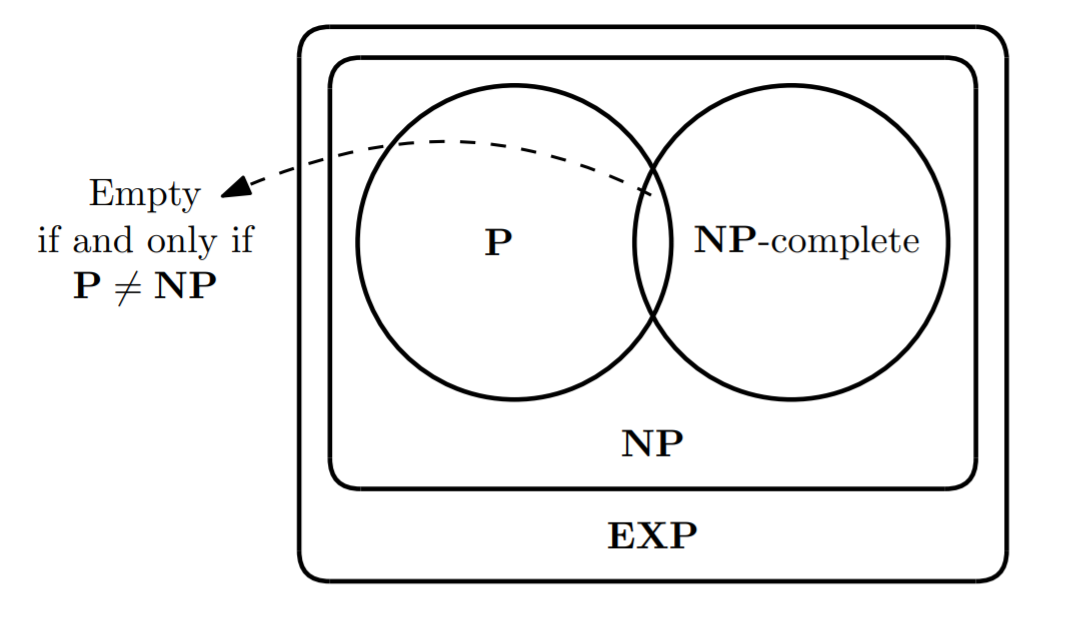
\includegraphics[width = \textwidth]{figures/P-NP-diagram.png}
	\caption{\( \P \subseteq \NP \subseteq \EXP\).
		It is not known whether \NP~and \P~are equal or different, same for \NP~and \EXP. We only know that $\P \neq \EXP$.}
	\label{fig:P-NP-diagram}
\end{marginfigure}


\section{The Cook-Levin Theorem}

\subsection*{Boolean formulas, CNF, and \SAT}

Some of the simplest examples of \NP-complete problems come from propositional logic. A \emph{Boolean formula} over the variables $u_1,\ldots,u_n$ consists of the variables and the logical operators AND ($\wedge$), OR ($\vee$), and NOT ($\neg$). For example, $(u_1 \wedge u_2) \vee (u_2 \wedge u_3) \vee (u_3 \wedge u_1)$ is a Boolean formula. If $\varphi$ is a Boolean formula over variables $u_1,\ldots,u_n$, and $z \in \{0,1\}^n$, then $\varphi(z)$ denotes the value of $\varphi$ when the variables of $\varphi$ are assigned the values $z$ (where we identify 1 with \textsc{True} and 0 with \textsc{False}). \emph{A formula $\varphi$ is satisfiable if there exists some assignment $z$ such that $\varphi(z)$ is \textsc{True}. Otherwise, we say that $\varphi$ is unsatisfiable.}

The above formula $(u_1 \wedge u_2) \vee (u_2 \wedge u_3) \vee (u_3 \wedge u_1)$ is satisfiable, since the assignment $u_1 = 1, u_2 = 0, u_3 = 1$ satisfies it. In general, an assignment $u_1 = z_1, u_2 = z_2, u_3 = z_3$ satisfies the formula iff at least two of the $z_i$'s are 1.

A Boolean formula over variables $u_1,\ldots,u_n$ is in \emph{CNF form} (shorthand for \emph{Conjunctive Normal Form}) if it is an AND of OR's of variables or their negations. For example, the following is a 3CNF formula: (here and elsewhere, $\overline{u_i}$ denotes $\neg u_i$)
\[
	(u_1 \vee \overline{u_2} \vee u_3) \wedge (u_2 \vee \overline{u_3} \vee u_4) \wedge (\overline{u_1} \vee u_3 \vee \overline{u_4})
\]
More generally, a CNF formula has the form
\[
	\bigwedge_i \left(\bigvee_j v_{ij}\right)
\]
where each $v_{ij}$ is either a variable $u_k$ or its negation $\overline{u_k}$. The terms $v_{ij}$ are called the \emph{literals} of the formula and the terms $(\bigvee_j v_{ij})$ are called its \emph{clauses}. A $k$CNF is a CNF formula in which all clauses contain at most $k$ literals. We denote by \SAT the language of all satisfiable CNF formulae and by \kSAT{3} the language of all satisfiable 3CNF formulae.


\begin{theorem}[Cook-Levin]
	The following two languages
	\begin{align*}
		\SAT     & = \{\llcorner F\lrcorner | F \text{ is a satisfiable CNF}\}  \\
		\kSAT{3} & = \{\llcorner F\lrcorner | F \text{ is a satisfiable 3CNF}\}
	\end{align*}
	are \textbf{NP-complete}.
	\label{thm:cook-levin}
\end{theorem}
\begin{proof}[sketch]
	The steps for proving Theorem~\ref{thm:cook-levin} are the following.
	Both \SAT~and \kSAT{3}~are clearly in \NP, since a satisfying assignment can serve as the certificate that a formula is satisfiable. Thus we only need to prove that they are \NP-hard. We do so by (a) proving that \SAT~is \NP-hard and then (b) showing that \SAT is polynomial-time Karp reducible to \kSAT{3}. This implies that \kSAT{3}~is \NP-hard by the transitivity of polynomial-time reductions. See e.g. Section 2.3 of \citet{Arora2009}.
\end{proof}

\section{Proving the hardness of a problem}

The only way to prove that a problem is hard is to prove the language is \NP-complete, in this way we have proven that the problem is not so hard (being in \NP) but not so easy either (unless $\P = \NP$ of course ).

But how can we prove that a language \(\lang{L}\) is \NP-complete?\\

If we want to prove $\lang{L}$ to be \NP-complete, we have to prove two statements:
\begin{enumerate}
	\item That $\lang{L}$ is in \NP.
	      \begin{itemize}[noitemsep,topsep=0pt,parsep=0pt,partopsep=0pt]
		      \item This amounts to showing that there are $p$ polynomial and $\mathcal{M}$ polytime TM such that $\lang{L}$ can be written as
		            $$\lang{L} = \{x \in \{0,1\}^* \mid \exists y \in \{0,1\}^{p(|x|)}.\mathcal{M}(x,y) = 1\}$$
		            which is typically rather easy.
	      \end{itemize}
	\item That any other language $\lang{H} \in$ \NP{} is such that $\lang{H} \leq_p \lang{L}$.
	      \begin{itemize}[noitemsep,topsep=0pt,parsep=0pt,partopsep=0pt]
		      \item We can of course prove the statement directly.
		      \item More often (e.g. when showing 3SAT \NP-complete), one rather proves that $\lang{J} \leq_p \lang{L}$ for a language $\lang{J}$ which is already known to be \NP-complete.
		      \item This is correct, simply because $\leq_p$ is transitive (Theorem~\ref{thm:pre-order-reduc-p=np})
		            \begin{gather*}
			            \vdots \\
			            \lang{H} \xrightarrow{\leq_p} \lang{J} \xrightarrow{\leq_p} \lang{L} \\
			            \vdots
		            \end{gather*}
	      \end{itemize}
\end{enumerate}

\section{Examples of \NP-complete problems}

\subsection{\INDSET}
The \textbf{Independent Set} of a graph $\mathbb{G}$ with vertex set $V$ and edges set $E$ defined as follows
\[
	\INDSET = \{ \langle \mathbb{G}, k \rangle : \exists S \subseteq V \text{ s.t. } |S| \ge k \text{ and } \forall u,v \in S, (u,v) \notin E\} \, .
\]
The Independent Set Problem is the problem of determining whether a graph $\mathbb{G}$ admits an independent set of size at least $k$.

\emph{input}: $(\mathbb{G},k)$\\
\emph{output}: $1$ iff \(\exists S \subseteq V\) s.t. \(|S|\geq k\) \(\land\) \(\forall v,u \in S\) \((v,u) \notin E\)


\subsection{\CLIQUE}
\[
	\CLIQUE = \{ \langle \mathbb{G}, k \rangle : \exists S \subseteq V \text{ s.t. } |S| \ge k \text{ and } \forall u,v \in S, u \neq v \implies (u,v) \in E \}
\]

\emph{input}: $(\mathbb{G},k)$\\
\emph{output}: 1 iff $\mathbb{G}$ contains clique of size $k$\\
A clique is a subset W \(\subseteq\) V of its vertices such that any pair v, w \(\in\) W  of distinct vertices is such that (v, w) \(\in\) E . In other words given an undirected graph a clique is a subset of this graph where all the vertices are connected, effectively yielding a complete subgraph.

\subsection{\kSAT{k}}
input: a formula F\\
output: 1 iff F is a satisfiable kCNF\\

\subsection{Vertex Cover or Node Cover}
\emph{input}: $(\mathbb{G},k)$\\
\emph{output}: 1 iff exists a subset of the vertices \(\exists C \subseteq V\) so that \(|C| \leq b\) and \(\forall (v,u) \in E. v\in C\ or\ u\in C\) \\
It means that a node cover of a graph G is a part of the vertices for which we know that at least one vertices for each node is in the cover.

\subsection{Universal Sink (US)}
For having an universal sink we need to have a \emph{directed} graph $\mathbb{G}=(V,E)$. Since we have a directed graph we do not require $E$ to be symmetric. We can represent graphs using the so-called adjacency matrix. So we can write the graph as the pair $\mathbb{G}=(V,A)$ where $A$ is a \(x \times x\) matrix over \binset. If we put a 1 in the position $i,j$ then we have a edge between the vertex $i$ and $j$.

\emph{input}: $\mathbb{G}$\\
\emph{output}: 1 iff exists a vertex \(v_i\) such that \(\forall j,k \leq n\) with \(j \neq i\) we have \(A_{i,k}=0\) and \(A_{j,i}=1\) .\\
It means that a directed graph has universal sink, (at max 1) if it has a vertex so that all the nodes goes into the vertex and nothing comes out of it.

\subsection{Set Packing (SP)}
\emph{input}: $(S_1,...,S_n,k)$\\
\emph{output}: 1 iff \(\exists  \, (P_1,P_2...,P_k) \in (S_1,...,S_n) \) s.t. \(\forall i,j \ i\neq j\ P_i \cap P_j = \emptyset\)  \\
It means that given a set of sets the problems gives 1 only if exists a subset of size k of this set so that every element (set) is independent from one another.

\subsection{Subgraph Isomorphism (SI)}
Given two undirected graphs \(\mathbb{G}_1 = (V_1,E_1)\) and \(\mathbb{G}_2 = (V_2,E_2)\) we say that:
\begin{enumerate}
	\item \(\mathbb{G}_1\) is a subgraph of \(\mathbb{G}_2\) if and only if \(V_1 \subseteq V_2\) and \(E_1 = E_2 \cap (V_1 \times V_1)\)
	\item A function \(h: V_1 \rightarrow V_2\) is a homomorphism from \(\mathbb{G}_1\) to \(\mathbb{G}_2\) if and only if (v,u)\( \in E_1\) implies \((h(v),h(u)) \in E_2\) .
	\item \(\mathbb{G}_1\) is isomorphic to \(\mathbb{G}_2\) if and only if there exists a bijective (function between the elements of two sets, where each element of one set is paired with exactly one element of the other set, and each element of the other set is paired with exactly one element of the first set.) homomorphism h from \(\mathbb{G}_1\) to \(\mathbb{G}_2\).
\end{enumerate}

\emph{input}: $\mathbb{G}_1 = (V_1,E_1)$ and $\mathbb{G}_2 = (V_2,E_2)$\\
\emph{output}: 1 iff $\mathbb{G}_1$ has a subgraph isomorphic to $\mathbb{G}_2$.

\subsection{SUBSETSUM (SSP)}
In its most general formulation, there is a multiset S of integers and a target-sum T, and the question is to decide whether any subset of the integers sum to precisely T.

